\documentclass[11pt,a4paper]{article}

\usepackage{graphicx}
\usepackage{listings}
\usepackage{color}
\usepackage[usenames,dvipsnames,svgnames,table]{xcolor}
\usepackage{multirow}


\newcommand{\adiossw}{\emph{ADIOS\_SELECTION\_WRITEBLOCK}}

\newcommand{\adiossb}{\emph{ADIOS\_SELECTION\_BOUNDINGBOX}}

\newcommand{\alac}{ALACRITY}

\newcommand{\shell}[1]{\$\{{#1}\}}



\begin{document}
\title{\alac\ Release Document}
\maketitle

\section{ \alac\ Introduction}

\subsection{What is \alac\ ?}


\alac\ is a lightweight query engine based on PForDelta compressed inverted indexes over scientific data. 
Its purpose is to accelerate response times on exploratory query-driven analysis and visualization. 
It is designed to function either during post processing or in situ (while a simulation application is running concurrently). 
Its core idea is to binning data based on significant bits in the IEEE floating-point representation and thus, the search space is reduced to a subset of bins by excluding bins that definitely are not in the querying condition.

The below sections give the details of \alac, in which Section~\ref{sec:alac-indexing} presents how \alac\ does the binning (referred as indexing) while Section~\ref{sec:alac-querying} describes how \alac\ answers queries based on indexed built previously.

\subsubsection{Indexing} 
\label{sec:alac-indexing}

\alac's speciality is for scientific data, which is floating-point values. 
The key observation is that, while floating-point datasets have a large number
of unique values, the highest $k$ bytes (significant bits) of the datasets typically have lower
cardinality (number of unique values) compared to the rest of the data.  
Thus, its core strategy is to binning on the high-order bytes/significant bits of the data, while storing the low-order bytes separately, and subsequently applying compression methods on resultant Inverted Indexes. 

\begin{figure}[ht]             
\begin{center}                 
    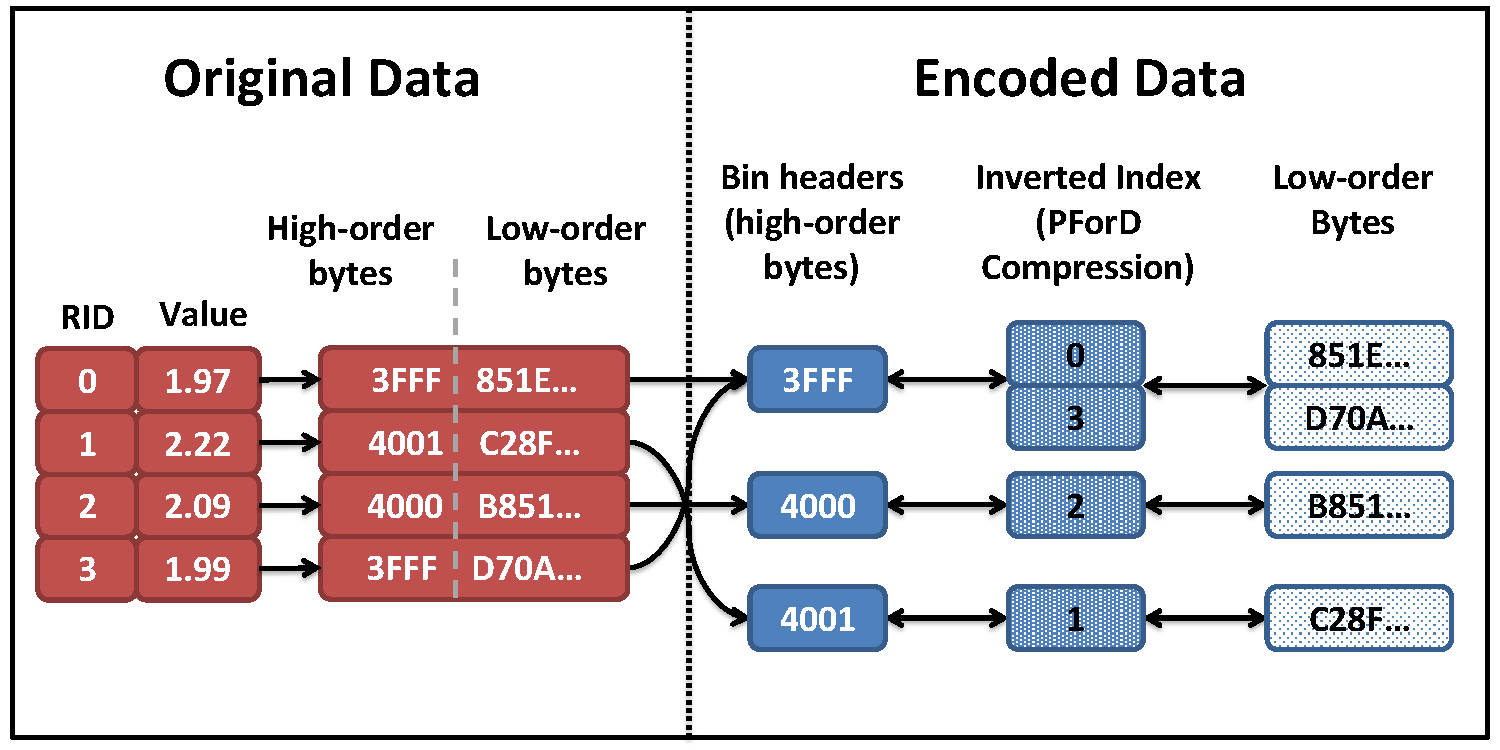
\includegraphics[width=0.80\textwidth]{figures/alacrity-encoding-overview-color}
\end{center}
\caption{An overview of how raw floating-point data is encoded by \alac\ for
compact storage and query-optimized access.}
\label{fig:alac_method}  
\end{figure}

Figure~\ref{fig:alac_method} demonstrates the significant-bit-based binning strategy (also referred as \emph{encoding}) employed in \alac. 
The input data is treated as a linear data array, and each data is implicitly associated with an Row ID (RID) starting with 0. 
Every data is examined under the two-part split, while the high-order bytes (significant bits) produce bins, in which RIDs of the same-bin data are organized into one bin (referred as inverted indexes), and low-order bytes bin are correspondingly concatenated as a low-order-byte bin. 
These inverted indexes are further compressed by the PForDelta compression method to reduce the storage footage. 

The implementation of the encoding method is the function \emph{ALEncode} defined in \emph{src\//ALEncode.c}. It has two scans. The first scan builds the bin layout (see the function \emph{determineBinLayout}) by counting the number of elements in each bin (all possible bins are enumerated at first). The second scan splits every data, and put its associated RID into the bin and its lower-order bytes data in the corresponding lower-order byte bin (see the function \emph{encodeWithInvertedIndex}). 

\emph{The command of build \alac\ indexes} Building \alac\ is relatively easy as we only need one single command. The command looks like this:

  \shell{ENCODE} encode -p\shell{PSIZE}E  -x -e\shell{DATA\_TYPE}  -s\shell{SIG\_BITS}  \shell{PATH\_TO\_ORIG\_DATA} \shell{PATH\_TO\_OUTPUT} 
  
  where \shell{ENCODE} is the path to the executable \emph{alac}, \shell{PSIZE} is the number of elements in each partition, \shell{DATA\_TYPE} could be \emph{double} or \emph{single} indicates whether the data is double or single floating point data, \shell{SIG\_BITS} is the number of significant bits used in the binning, \shell{PATH\_TO\_ORIG\_DATA} is the path to the original data which is a binary binary (unfortunately, that is the only input data format \alac\ now supports), and the \shell{PATH\_TO\_OUTPUT} is the path to the index output.
  Additionally, \emph{-x} indicates inverted indexes are compressed by the PForDelta compression. If you want inverted indexes without any compression, please replace \emph{-x} with \emph{-i}.
  
  Notice that there is an partition option in the encoding command, this is because \alac\ divides entire original input data into partitions to prevent the overflow. It works well for extreme large datasets. Yet, it also has an shortcoming, that is the number element of one partition can not exceed $2^{32}$ since the internal data type of RID is \emph{uint32\_t}. 
  In addition, there are other ways of specific the partition size, I do not cover them for the sake of space. Please refer to the \emph{alacrity.c} in \emph{tools} folder for details. 
  
  Blow is an example of encoding command. It means encoding the original double precision data using 16 significant bits with PForDelta compression, and each partition has 20 millions elements. One more thing I would like to point out is that the \shell{PATH\_TO\_OUTPUT} has the prefix (in this case, it is \emph{temp}), and temp-compressed\_data.dat (low-order byte data), temp-metadata.dat (\alac's metadata), and temp-query\_index.dat (inverted index either compressed or non-compressed) are generated. 
  
  build/bin/alac encode -p20000000E -x -edouble -s16 /home/chris/temp.bin /home/chris/temp
  
  
\subsubsection{Querying}
\label{sec:alac-querying}

\alac's querying ability supports RID-retrieval queries with multi-variate constraints  (e.g., select \emph{RIDs} from \emph{ALACRITY-format indexes} where  \emph{5 $<$  temperature $<$ 18} and \emph{20 $\le$ pressure $<$ 60}) . 
Differ from the query APIs designed in ADIOS (see Section~\ref{sec:alac-adios-apis} for details), it does not support a spatial constraint. 
To understand the \alac\ query processing, we first present the query processing for uni-variate query (e.g., select \emph{RIDs} from \emph{ALACRITY-format indexes} where  \emph{5 $<$  temperature $<$ 18}), which is explained step by step below with the flowchart (Figure~\ref{fig:alac-uniquery}). 


\begin{figure}[ht]             
\begin{center}                 
    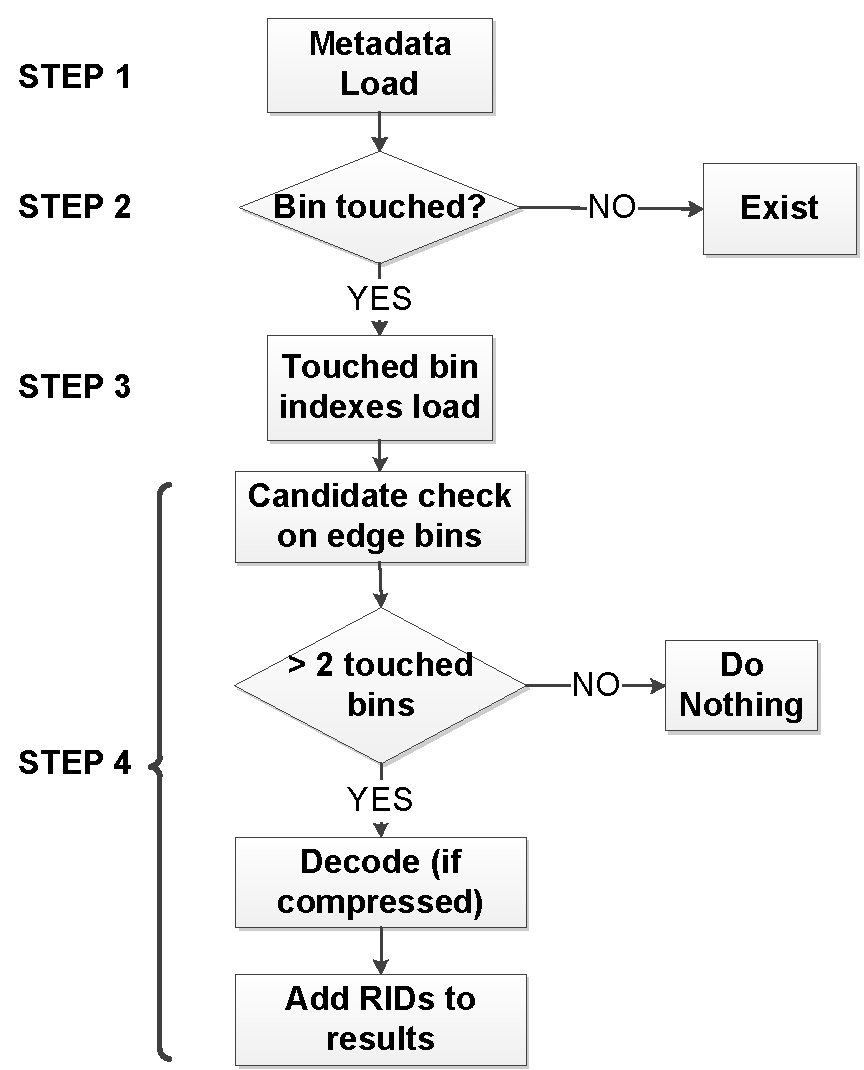
\includegraphics[width=0.80\textwidth]{figures/uniquery-alac}
\end{center}
\caption{A flowchart of \alac's query processing for uni-variate queries}
\label{fig:alac-uniquery}  
\end{figure}


\begin{enumerate}
\item \alac\ metadata load 
Loading \alac's metadata is an beginning step and it mainly reads the bin layout information created during the encoding step. Please see the details in the function \emph{getPartitionMetadata}. 

\item Bin ``touching'' determination

Use the input value query constraint to determine how many bins falls in the value constraint (see function \emph{findBinRange1C}). 
If there is no bin touching, program exists; otherwise, proceeds to next step. 

\item ``Touched'' bins' indexes load

Read indexes (either compressed or uncompressed) for every ``touched'' bin (see the function \emph{ALPartitionStoreReadIndexBins})

\item Filter RIDs from ``touched'' bins

At this step, it outputs resultant RIDs based on ``touched'' bins. 
There are two categories bins among in ``touched'' bins. 
One type of bin is edge bins, which are top and bottom bins in the ``touched'' bin list and require to be further examined (refereed as \emph{candidate check}). 
The reason is that some RIDs might not in the resultant RID list. 
And the criteria of the determination depends on whether the corresponding value satisfies the query constraint or not. 
Another type of bin is internal bins, which are bins except edge bins, and do not need the further examination, meaning all RIDs in these internal bins go to the results.
Additionally, internal bins only exist if only the number of ``touched'' bins is more than 2. 
For example, if bin 3, 4, 5 and 6 are ``touched'' bins, bin 3 and 6 are \emph{edge} bins need to be examined, and bin 4 and 5 are internal bins. 
Note that if bins are in compressed format, the decompression occurs before. 
In addition, in the \emph{candidate check} step (see the function \emph{candidateCheck}), the original data is first recovered first by assemble the high-order and low-order bytes (see the function \emph{readAndReconstituteData}) and the query constraint is applied on the recovered data during the scan. 
\end{enumerate}

Now, we move on to the query processing for multi-variate queries, in which a temporal result obtained from processing one query constraint is represented by a bitmap. 
These bitmaps are performed by bitwise operations (depends on the keywords, i.e., AND, OR, and NOT) after all query constraints are processed. 
Note that processing one query constraint is almost same as the univariate query processing, except in the last step, it outputs a bitmap, rather than RIDs, which requires an additional step to sets RID in the bitmap. 
Figure~\ref{fig:alac-multiquery} shows overview of the multi-variate query processing, please check the \emph{tools\//multiquery.c} for details.  
As mentioned, the step 1 in the Figure~\ref{fig:alac-multiquery} is replaced with uni-variate query processing. 

\begin{figure}[ht]             
\begin{center}                 
    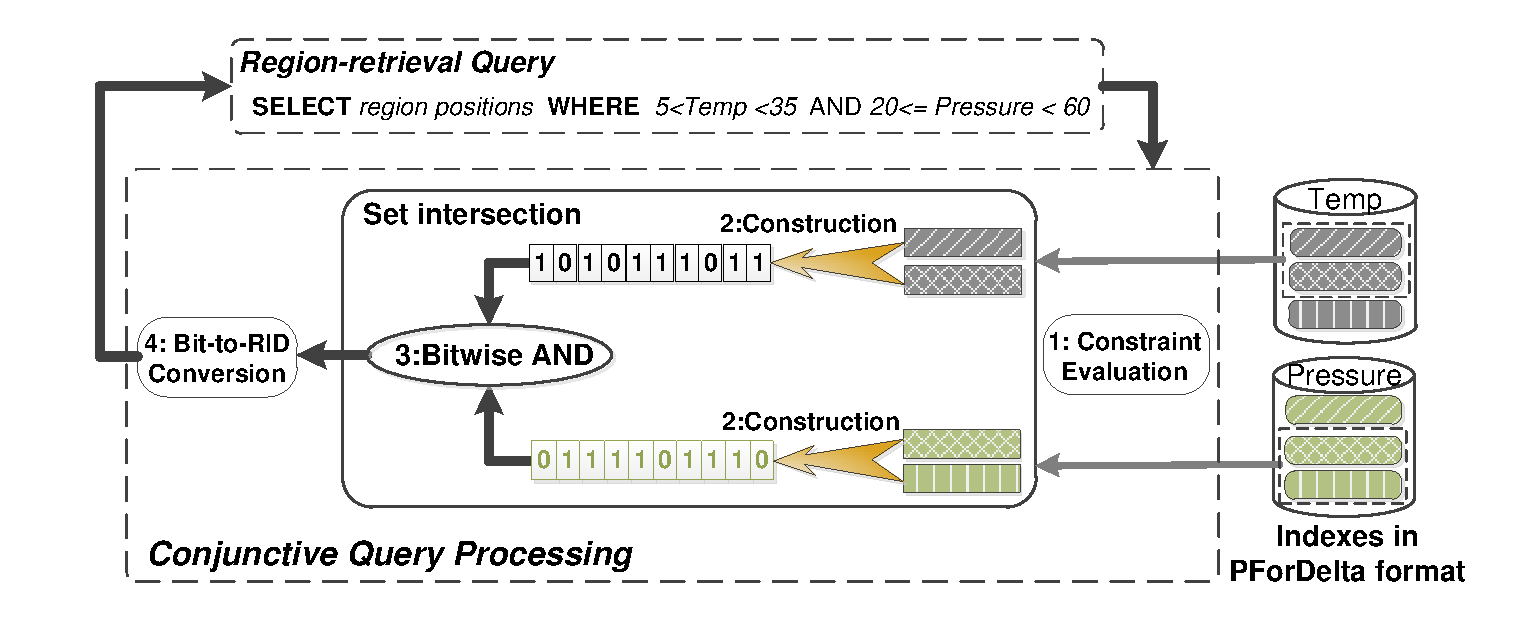
\includegraphics[width=0.90\textwidth]{figures/set-intersection-overview}
\end{center}
\caption{An overview of multi-variate query processing, which is composite of multiple independent univariate query processing through bitmaps. }
\label{fig:alac-multiquery}  
\end{figure}

%\subsubsection{Utility Tools}

%\subsubsection{Software Build}

\section{\alac\ within ADIOS Introduction}

\subsection{How does \alac\ within ADIOS differ from \alac\ alone?}
There are three main differences between the pure \alac\ and \alac\ within ADIOS, they are: 
\begin{enumerate}
\item The query APIs designed in ADIOS is more complicated than the query interface in pure \alac\. 
Specifically, the query APIs not only have value constraints, but also a spatial constraint ( denoted as input bounding box $B$). 
Note that the spatial constraint could be a \adiossw, but for illustration purpose, I only use the \adiossb\ since the process of \adiossw\ is similar to that of \adiossb.
In addition, the query APIs returns coordinates to users, in which the returning coordinates are relative to input bounding box $B$ and they are retrieved in multi-batch manner. 

\item The index building of \alac\ within ADIOS is accomplished through ADIOS transformer layer, which means the index building is achieved in \emph{in situ} fashion (while the data is writing out by the application, the index is built at the same time), as oppose to a post-processing manner in the pure \alac\. 
This also means the \alac\ indexes are stored in BP format in contrast to binary file format in pure \alac\. 
To the developer, the discrepancy of index format causes different APIs of reading data (especially meta, indexes, and low-order bytes data) from \alac.


\item The differences of query processing in \alac\ within ADIOS are primarily caused from the ADIOS query APIs, besides the different APIs of reading \alac\ data. 
In particularly, the query processing in \alac\ within ADIOS has to deal with the spatial constraint, ensuring the resultant coordinates to being in the input bounding box $B$. 

 
\end{enumerate}

Sections below document details of each point.  Unless otherwise stated, \alac\ below refers to the \alac\ within ADIOS. 
In addition,  all source codes mentioned below refer to codes in \emph{src\//query\//query\_alac.c}, except source codes in section~\ref{sec:transform-index-build} refer to codes in \emph{src\//transforms\//adios\_transform\_alacrity\_write.c}.

\subsubsection{APIs}
\label{sec:alac-adios-apis}
There are two main aspects \alac\ responds to ADIOS query APIs worth to detail. 
\begin{enumerate}
\item query-compose APIs

As ADIOS query APIs allow end-users to compose queries with different value constraints. The \alac\ internally has a tree structure to represent each individual query constraint and the composition relation between individual query constraints relying on \emph{ADIOS\_QUERY} structure defined in \emph{adios\_query.h}. 
The tree structure is processed in bottom-up fashion recursively, and each individual query is processed independently (please refer to the function \emph{adios\_alac\_process})

\item the result-retrieval API

End-users can retrieve resultant coordinates computed by \alac\ in batch manner, which means a desired number of results is specified by end-users. 
To achieve this functionality, the \alac\ internally represents final results with a uncompressed bitmap structure (basically, it is an array of \emph{uint64\_t}. please see the \emph{ADIOS\_ALAC\_BITMAP} structure. 
The reason for using the bitmap is that it has fast speed of processing query keywords (i.e., AND, OR and NOT), which is achieved by corresponding bitwise operations. 
In addition to the bitmap itself, we track the position of results so far are retrieved by users. 
This position is indicated by the field (\emph{lastConvRid}) in the \emph{ADIOS\_ALAC\_BITMAP} structure.
Note that \alac\ does not keep the status of the \emph{ADIOS\_ALAC\_BITMAP} structure, instead we let the user to keep it. 
This information is kept in the field \emph{queryInternal} of  \emph{ADIOS\_QUERY} structure.
The conversion and de-conversion between them are performed by functions \emph{convertALACBitmapTomemstream} and  (convertMemstreamToALACBitmap), respectively.

One last thing I would like to point out is the bitmap-to-coordinates conversion. 
There is a discrepancy between the internal represent structure (i.e., bitmap) and user-desired data structure (i.e., coordinates), so we need to convert the bitmap to the coordinates, which is achieved by the function \emph{adios\_query\_alac\_retrieval\_pointsNd}.
The basic idea of this function is that we first move the position from last retrieval, read next $N$ (where $N$ is the user-specified batch retrieval size) bits, and convert all 1 bits to the coordinates. 
The conversion is performed by keeping dividing the RID (the position of an one bit sits) by the highest dimension (dimensions that changes fastest) in the function (\emph{ridToCoordinates}).

\end{enumerate}

\subsubsection{Index Building}
\label{sec:transform-index-build}

As mentioned, the \alac\ index is built through transformer layer, which is seen in \emph{src\//transforms\//adios\_transform\_alacrity\_write.c}
The basic idea (shown in the function \emph{adios\_transform\_alacrity\_apply}) is that when the transformer layer receives data from upper layers, it first parse the XML to obtain the configuration of \alac\ index building (i.e., the number of significant bits, compression method to compress the RIDs, and whether keeps the lower-order bytes or the original data) and it then invokes the index build function (\emph{ALEncode}, provided by the pure \alac) to build indexes. 

List~\ref{sample-s3d} shows an example of showing input configurations for building \alac\ indexes. The key component in this sample xml file is the ``\emph{transform}'' tag, whose value begins with \emph{alacrity}, following by several key-value pairs. Table~\ref{table:index-build-conf} has a list of keys associate with \alac\ index build.  
The source code of parsing the configuration is shown in the function \emph{parse\_configuration}.

As a result of this index building, every PG within BP file contains \alac\ metadata, indexes, lower-order-byte data (if enabled) and original data (if enabled).

\begin{table}
\begin{tabular}{ |l|l|l| }
\hline

KEY & VALUE & COMMENT \\ \hline
\multirow{2}{*}{IndexForm} & ALInvertedIndex & Inverted index, no compression\\
 & ALCompressedInvertedIndex & Inverted index, with PForDelta compression \\ \hline
\multirow{1}{*}{sigBits} & number less than 64 & number of significant bits\\ \hline
\multirow{2}{*}{loBytes} & true & keep low-order-bytes\\
 & false & do not keep low-order-bytes \\
\hline
\multirow{2}{*}{origData} & true & keep original data \\
 & false & do not keep original data  \\
\hline
\end{tabular}
\caption{Configurable options of \alac\ index build via transformer layer}
\label{table:index-build-conf}
\end{table}

 \lstset{
    language=xml,
    tabsize=3,
    %frame=lines,
    caption=Sample configurable XML for \alac\ index building,
    label=code:sample,
    frame=shadowbox,
    rulesepcolor=\color{gray},
    xleftmargin=20pt,
    framexleftmargin=15pt,
    keywordstyle=\color{blue}\bf,
    commentstyle=\color{OliveGreen},
    stringstyle=\color{red},
    numbers=left,
    numberstyle=\tiny,
    numbersep=5pt,
    breaklines=true,
    showstringspaces=false,
    basicstyle=\footnotesize,
    emph={transform},emphstyle={\color{magenta}},
    label=sample-s3d}
    \lstinputlisting{ref/sample-s3d.xml}	

\subsubsection{Query Processing}
As mentioned earlier, every individual query constraint is processed independently. 
Therefore, we only present processing steps for one query constraint, which is seen in the function \emph{adios\_alac\_uniengine}. 
In addition, the process for the \adiossb\ is similar to the \adiossw. 
I present the query process only for \adiossb\ for simplicity.
The idea is that for every query constraint processing, we first create an uncompressed bitmap, the presence of 1s represents the corresponding coordinates in the temporal results. 
We then compute the ``touched'' PGs (referred as candidate PGs) by invoking the function \emph{adios\_find\_intersecting\_pgs} provides from the transformer layer. 
In other words, the \emph{adios\_find\_intersecting\_pgs} function returns PGs are overlapping or fully contained in the input bounding box $B$, and discarding PGs not disjoint with $B$.
Last, every PG in the candidate PG set are further examined to find exact results for the given query constraint. 
This is where the complexity comes from, and the implementation is seen at the function \emph{proc\_write\_block}.

Now, I present the logic in the function \emph{proc\_write\_block} step by step. 
\begin{enumerate}
\item load \alac\-plugin metadata by the function \emph{read\_alacrity\_transform\_metadata} provided by the transformer layer. As indexes are built within the transformer layer, it makes sense the query processing has to interactive with transformer layer to obtain any \alac\ related information. 

\item \alac\-plugin metadata load

Load \alac\ metadata by the function \emph{readPartitionMeta} to specific \alac\ information, such as the bin layout and indexes. 

\item Bin ``touching'' determination
This is the same as the step in the Section~\ref{sec:alac-querying}. If there is no bin, continue to process the next PG. Otherwise, proceeds to the next step.

\item PG-fully-contained determination

Use ADIOS statistics information to determine whether the whole PG is fully contained in query constraints (both in spatial and value aspects). This step only applies when the resultant bins from the previous step span the entire bin. 

\item ``Touched'' bins' indexes load

This is the same as the step in the Section~\ref{sec:alac-querying}. 
But this time, the indexes are read from transformed format, see the function \emph{readIndexAmongBins} for details.
In addition, the next step branches out depending on whether indexes are compressed or not. Yet, since the scenario of index compressed is more complicated than that of index uncompressed, I only present the index compression case. 

\item Decode RIDs of a whole PG to the bitmap

If a PG is fully contained,  we can avoid the index decode step (i.e., decoding the compressed RIDs to RIDs) by taking advantages of the fact that is all RIDs need to be set. 
In other words, we rely on the prior knowledge that all RIDs must be RIDs from 0 to $R$, where $R = $ \emph{PG\_size} -1, which explains the reason why we do not need to decode the compressed RIDs. 

Additionally, we notice that RIDs that are on dimension that changes fastest are consecutive. 
We take this as another advantage, which allows us to set a consecutive 1 bits in the bitmap (see function \emph{set\_consecutive\_bits}). 

Last, I would like to point out is that in the current implementation, this is implemented only for data up to 3 dimensions, which are the most common dimensionalities.
Functions \emph{setBits\_for\_wholePG\_1\_2\_dim} and \emph{setBits\_for\_wholePG\_3\_dim} are current implementation for 1 or 2 dimensions and 3 dimensions, respectively. 
The reason I have functions for different dimensions is that the stride between two consecutive bits depends on the dimensionality, making it hard to generalize. 
If dimensionality is higher than 3, we go back to original routine, (function \emph{ALDecompressRIDtoSelBox}), which involves three tedious conversion (i.e., compressed RIDs to RIDs, RIDs to coordinates within $B$ and coordinates to RIDs within $B$).


\item Set the bitmap for ``touched'' bins

There are two categories bins among on ``touched'' bins. 
One type of bin is edge bins, which are top and bottom bins in the ``touched'' bin list and require to be further examined. 
Another type of bin is internal bins, which are bins except edge bins, and do not need the further examination. 
This is same as the pure \alac. 

With regard to edge bins, we do a candidate check to determine which RIDs are in the result and which are not (see the function \emph{adios\_alac\_check\_candidate}). 
The major steps in the candidate check involves original data recovery and linear data scan (determining which value satisfies the query constraint or not), same as before. 
Note that if the value does satisfy the query constraint, it needs to be reflect in the bitmap with its RID. 
And the bitmap set requires the RID-Coordinate-RID conversion (see the function \emph{ridConversionWithoutCheck}). 
Furthermore, if current PG is partially overlaps with $B$, during the conversion, we need to do additional check, discarding those RIDs that are outside of $B$ (see the function \emph{ridConversionWithCheck}).

Whereas, for the internal bins, we set the bitmap by RIDs in bins. Here comes a second optimization, which aims for reduces the number of relatively expensive division and multiplication operations involved in the RID-Coordinate-RID conversion. 
This optimization is implemented by functions \emph{deltaBitSetsWithPGPartialCoveredCorderIn3D} and \emph{deltaBitSetsWithPGCoveredCorderIn3D}. 
The idea is to avoid the conversion for every RID by taking advantage of the current new RID based on the previous computed new RID is able to be calculated by addition operations.
Again, because the stripe of consecutive RIDs depends on the dimensionality, we have to make case by case for each dimension. 
\end{enumerate}

\section{Performance}

\subsection{Setup}
We have performed all experiments on the Edison machine. 
And the test data we used is the S3D bp file with 200 PGs. 
In addition, all data is stored on GFS file system.

\subsection{Indexing Performance}
We have two performance metrics, index size and index building time in parallel. 



\begin{figure}[ht]             
\begin{center}                 
    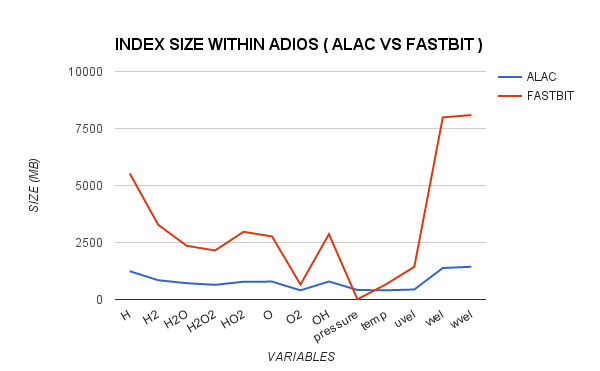
\includegraphics[width=0.90\textwidth]{figures/perf/alac-adios/idx-size-comp}
\end{center}
\caption{Index size comparison. In the ALACRITY index building, 24 significant bits are used on variable pressure and 16 significant bits are used on rest variables. Additionally, original data are discarded.  }
\label{fig:idx-size}  
\end{figure}




\begin{figure}[ht]             
\begin{center}                 
    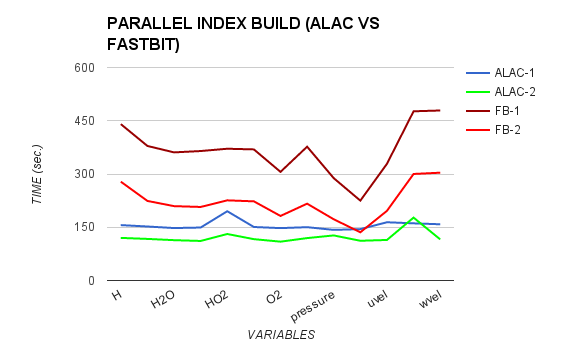
\includegraphics[width=0.90\textwidth]{figures/perf/alac-adios/parallel-idx-build-1}
\end{center}
\caption{Index building speed comparison using 1 and 2 processes.}
\label{fig:idx-build-1}  
\end{figure}


\begin{figure}[ht]             
\begin{center}                 
    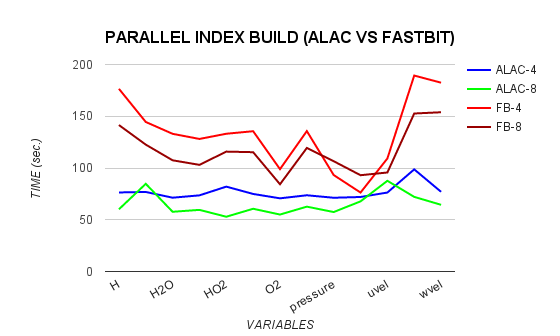
\includegraphics[width=0.90\textwidth]{figures/perf/alac-adios/parallel-idx-build-2}
\end{center}
\caption{Index building speed comparison using 4 and 8 processes.}
\label{fig:idx-build-2}  
\end{figure}


\subsection{Query Performance}

\subsubsection{Univariate Query}

\begin{figure}[ht]             
\begin{center}                 
    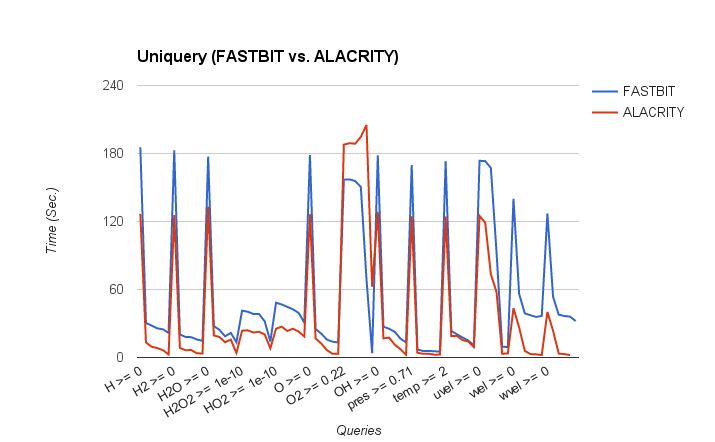
\includegraphics[width=0.90\textwidth]{figures/perf/alac-adios/uniquery-whole-space}
\end{center}
\caption{Performance comparison for univariate query with the \emph{whole} spatial selection.}
\label{fig:uniquery-whole}  
\end{figure}


\begin{figure}[ht]             
\begin{center}                 
    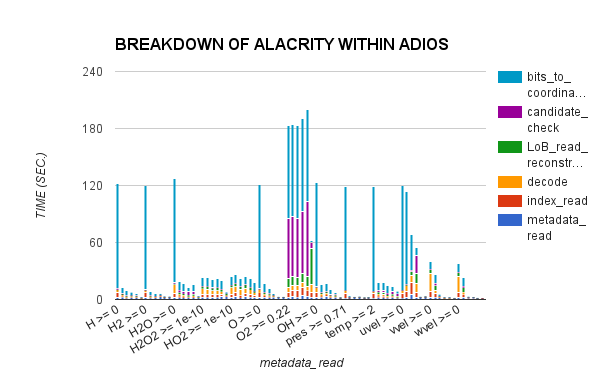
\includegraphics[width=0.90\textwidth]{figures/perf/alac-adios/breakdown-uniquery-whole-space}
\end{center}
\caption{Breakdown performance comparison for univariate query with the \emph{whole} spatial selection.}
\label{fig:uniquery-whole-breakdown}  
\end{figure}



\begin{figure}[ht]             
\begin{center}                 
    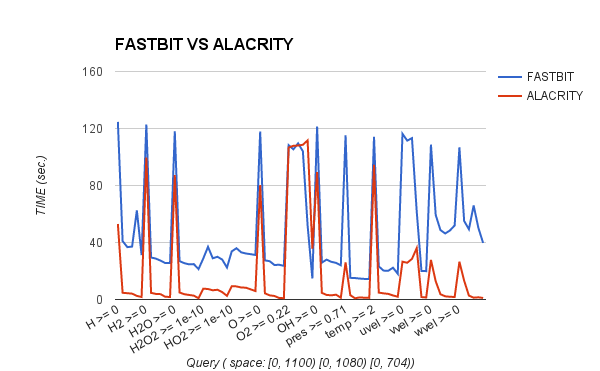
\includegraphics[width=0.90\textwidth]{figures/perf/alac-adios/uniquery-half-space}
\end{center}
\caption{Performance comparison for univariate query with the \emph{half} spatial selection.}
\label{fig:uniquery-half}  
\end{figure}


\begin{figure}[ht]             
\begin{center}                 
    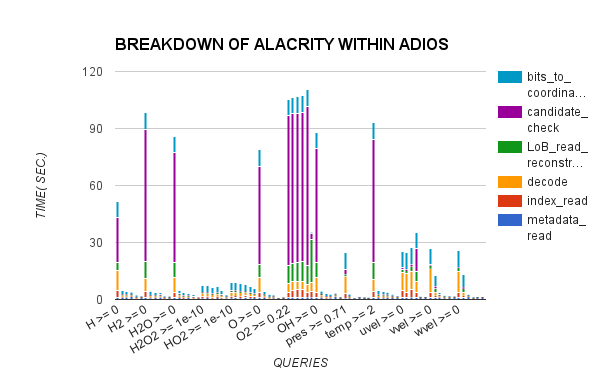
\includegraphics[width=0.90\textwidth]{figures/perf/alac-adios/breakdown-uniquery-half-space}
\end{center}
\caption{Breakdown performance comparison for univariate query with the \emph{half} spatial selection.}
\label{fig:uniquery-half-breakdown}  
\end{figure}




\begin{figure}[ht]             
\begin{center}                 
    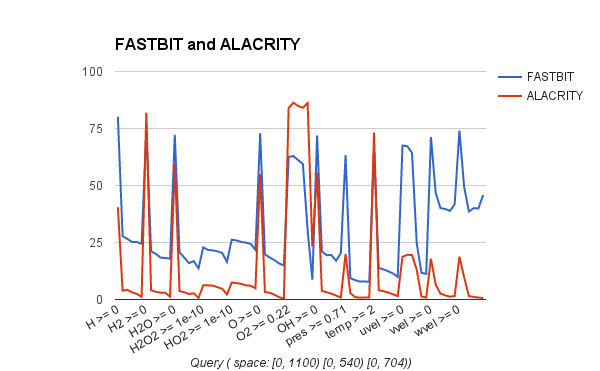
\includegraphics[width=0.90\textwidth]{figures/perf/alac-adios/uniquery-quarter-space}
\end{center}
\caption{Performance comparison for univariate query with the \emph{quarter} spatial selection.}
\label{fig:uniquery-quarter}  
\end{figure}


\begin{figure}[ht]             
\begin{center}                 
    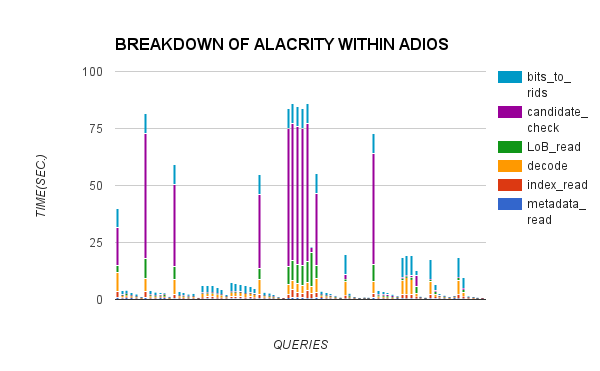
\includegraphics[width=0.90\textwidth]{figures/perf/alac-adios/breakdown-uniquery-quarter-space}
\end{center}
\caption{Breakdown performance comparison for univariate query with the \emph{quarter} spatial selection.}
\label{fig:uniquery-quarter-breakdown}  
\end{figure}




\begin{figure}[ht]             
\begin{center}                 
    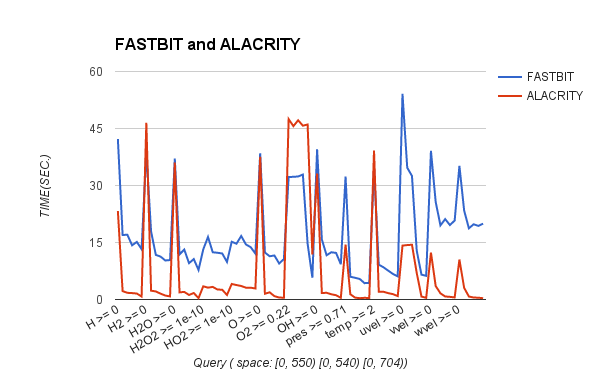
\includegraphics[width=0.90\textwidth]{figures/perf/alac-adios/uniquery-eighth-space}
\end{center}
\caption{Performance comparison for univariate query with the \emph{eighth} spatial selection.}
\label{fig:uniquery-eighth}  
\end{figure}


\begin{figure}[ht]             
\begin{center}                 
    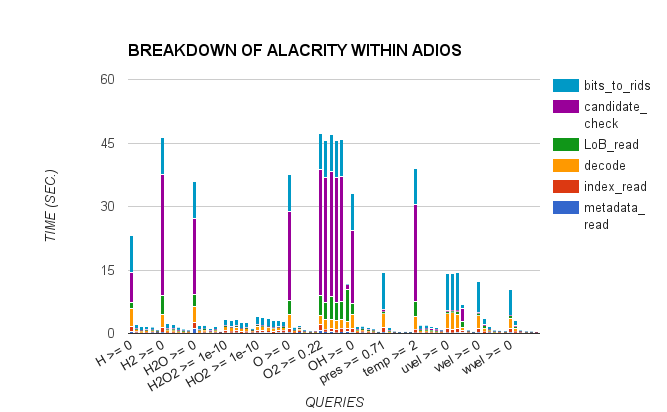
\includegraphics[width=0.90\textwidth]{figures/perf/alac-adios/breakdown-uniquery-eighth-space}
\end{center}
\caption{Breakdown performance comparison for univariate query with the \emph{eighth} spatial selection.}
\label{fig:uniquery-eighth-breakdown}  
\end{figure}


\subsubsection{Multivariate Query}



\begin{figure}[ht]             
\begin{center}                 
    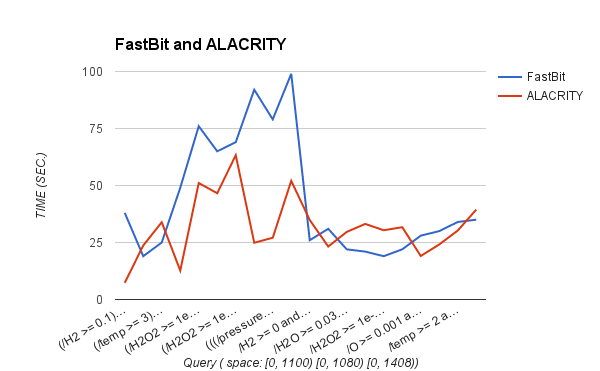
\includegraphics[width=0.90\textwidth]{figures/perf/alac-adios/multi-query-whole-space}
\end{center}
\caption{Performance comparison for multivariate query with the \emph{whole} spatial selection.}
\label{fig:multi-query-whole-space}  
\end{figure}


\begin{figure}[ht]             
\begin{center}                 
    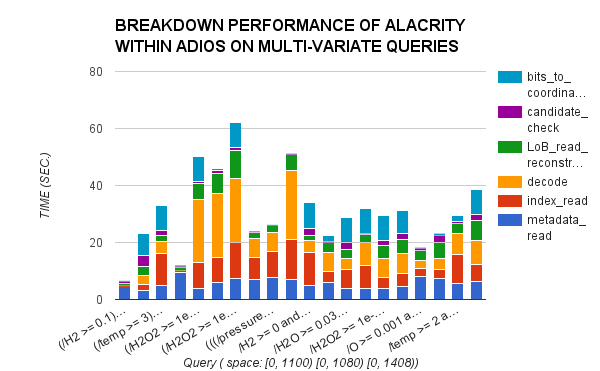
\includegraphics[width=0.90\textwidth]{figures/perf/alac-adios/breakdown-multi-query-whole-space}
\end{center}
\caption{Breakdown performance comparison for multivariate query with the \emph{whole} spatial selection..}
\label{fig:multi-query-whole-space-breakdown}  
\end{figure}


\end{document}